%%%%%%%%%%%%%%%%%%%%%%%%%%%%%%%%%%%%%%%%%%%%%%%%%%%%%%%%%%%%%%%%%%%%%%%%
% Copyright (c) 2023 The authors
%
% This work is licensed under a
% Creative Commons Attribution-ShareAlike 4.0 International License.
%
% You should have received a copy of the license along with this
% work. If not, see <http://creativecommons.org/licenses/by-sa/4.0/>.
%%%%%%%%%%%%%%%%%%%%%%%%%%%%%%%%%%%%%%%%%%%%%%%%%%%%%%%%%%%%%%%%%%%%%%%%


%%%%%%%%%%%%%%%%%%%%%%%%%%%%%%%%%%%%%%%%%%%%%%%%%%%%%%%%%%%%%%%%%%%%%%%%%%
%% Supplementary material
%%%%%%%%%%%%%%%%%%%%%%%%%%%%%%%%%%%%%%%%%%%%%%%%%%%%%%%%%%%%%%%%%%%%%%%%%%

\section{Model choice and implementation details}

\subsection{Label switching}\label{app:label-switching}

A well-known issue that arises when using MCMC methods in mixture-like models such as the one proposed in this work is \textit{label switching}, which in short refers to the non-identifiability of the components of the model caused by their interchangeability. In our case, this happens because the likelihood is symmetric with respect to the ordering of the component parameters \(b\) and \(\tau\), that is, \(\pi(Y|X,\theta)=\pi(Y|X, \nu(\theta))\) for any permutation \(\nu\) that rearranges the indices \(j=1,\dots, p\). Thus, since the components are arbitrarily ordered, they may be inadvertently exchanged from one iteration to the next in a MCMC algorithm. This can cause nonsensical answers when summarizing the marginal posterior distributions to perform inference, as different labelings might be mixed on each component \citep{stephens2000dealing}. However, this phenomenon is perhaps surprisingly a condition for the convergence of the MCMC method: as pointed out by many authors \citep[e.g.][]{celeux2000computational}, a lack of switching would indicate that not all modes of the posterior distribution were being explored by the sampler. For this reason, many ad-hoc solutions revolve around post-processing and relabeling the samples to eliminate the switching effect, but they generally do not prevent it from happening in the first place.

The most straightforward solutions consist on imposing an artificial identifiability constraint on the parameters to break the symmetry of their posterior distributions; see \citet{jasra2005markov} and references therein. A common approach that seems to work well is to simply enforce an ordering in the parameters in question, which in our case would mean requiring for example that \(\beta_i < \beta_j\) for \(i < j\), or the analogous with the times in \(\tau\). We have implemented a variation of this method described in \citet{simola2021approximate}, which works by post-processing the samples and relabeling the components to satisfy the order constraint mentioned above, choosing either \(b\) or \(\tau\) depending on which set of ordered parameters would produce the largest separation between any two of them (suitably averaged across all iterations of the chains). This is an area of ongoing research, and thus there are other, more complex relabeling strategies, both deterministic and probabilistic. A summary of several such methods can be found for example in \citet{rodriguez2014label} and \citet{papastamoulis2015label}.

\subsection{Selection of hyperparameters}\label{app:hyperparameters}

One of the key decisions in our Bayesian modeling scheme was whether to consider the number of components \(p\) as a member of the parameter space and integrate it into the model. While theoretically we could impose a prior distribution on \(p\) as well (e.g.\ a categorical distribution with a fixed maximum value), we found that this would have some unwanted practical implications. For instance, it would make the implementation more complex, since the dimensionality of the parameters \(b\) and \(\tau\) would need to be fixed at a certain maximum value beforehand, but the working value of \(p\) within the MCMC algorithm would vary from one iteration to the next. In this case we would have no immediate way of tracking down which set of parameters is ``active'' at any given time. A simple approach would be to always consider the first \(p\) parameters and ignore the rest, and we did indeed try this technique, but it gave rise to new difficulties and the results obtained were not good. In fact, the label switching issue is accentuated when \(p\) is allowed to vary \citep[c.f.][Section~2.3]{grollemund2019bayesian}, and on top of that, the interpretation of, say, the first coefficient \(\beta_1\) in a model with \(3\) components is different from the interpretation of the same coefficient in a model with only \(2\) components.

This inconsistency in the interpretation of the components when the dimensionality of the model increases or decreases could be mitigated using a particular type of MCMC method known as reversible-jump MCMC \citep{green1995reversible}. Theoretically, these algorithms are specifically designed to approximate the posterior distribution in mixture-like models when the number of components is unknown, allowing the underlying dimensionality to change between iterations. However, since they are not yet widely adopted in practice and a reference implementation is not available, we decided against using them in our applications. Another possibility would be to adapt a purely Bayesian model selection technique to our framework \citep[see][]{piironen2017comparison, gelman2013bayesian}, or even derive some model aggregation methods to combine the posterior distributions obtained for different-sized models. These methods are usually based in computing a quantity known as the \textit{Bayes factor}, which in turn requires the specific value of the normalizing integral constant we have been trying to avoid all along. In the end, for the sake of simplicity we decided to let \(p\) be a hyperparameter, so that we could use any model selection criteria (e.g.\ BIC, DIC or cross-validation) to select its optimal value.

As for the default values of the rest of hyperparameters in the prior distributions we propose, several comments are in order:
\begin{itemize}
    \item For the expected value \(b_0\) we propose to use the MLE of \(b\). Although the likelihood function is rather involved, an approximation of the optimal value is enough for our purposes. Our numerical studies suggest that the results are much better with this choice than, say, with a random or null vector.
    \item We found that the parameter \(g\) does not have as much influence on the final result, and the experimentation indicates that \(g=5\) is a good enough value.
    \item Lastly, we observed that the choice of \(\eta\) can have a considerable impact on the final predictors. This is why, in an effort to normalize its scale, we consider a compound parameter \(\eta = \tilde \eta \lambda_{\max}(\mathcal X_\tau^T \mathcal X_\tau)\), where \(\lambda_{\max}(\mathcal X_\tau^T \mathcal X_\tau)\) is the largest eigenvalue of the matrix \(\mathcal X_\tau^T \mathcal X_\tau\), and \(\tilde\eta > 0\) is the actual tuning parameter (which can be selected for instance by cross-validation strategies). This standardization technique has been used previously in the literature; see for example \citet{grollemund2019bayesian}.
\end{itemize}

\subsection{Affine-invariant ensemble sampler}\label{app:ensemble-sampler}

An interesting and often desirable property of MCMC sampling algorithms is that they be \textit{affine-invariant}, which means that they regard two distributions that differ in an affine transformation, say \(\pi(x)\) and \(\pi_{A, b}(Ax + b)\), as equally difficult to sample from. This is useful when one is working with very asymmetrical or skewed distributions, for an affine transformation can turn them into ones with simpler shapes. Generally speaking, a MCMC algorithm can be described through a function \(R\) as \(\Lambda(t+1)=R(\Lambda(t), \xi(t), \pi)\), where \(\Lambda(t)\) is the state of the chain at instant \(t\), \(\pi\) is the objective distribution, and \(\xi(t)\) is a sequence of i.i.d.\ random variables that represent the random behavior of the chain. With this notation, the affine-invariance property can be characterized as \(R(A\lambda+b, \xi(t), \pi_{A,b}) = AR(\lambda, \xi(t), \pi) + b\), for all \(A,b\) and \(\lambda\), and almost all \(\xi(t)\). This means that if we fix a random generator and run the algorithm twice, one time using \(\pi\) and starting in \(\Lambda(0)\) and a second time using \(\pi_{A,b}\) with initial point \(\Gamma(0)=A\Lambda(0)+b\), then \(\Gamma(t)=A\Lambda(t)+b\) for all \(t\). In \citet{goodman2010ensemble} the authors consider an ensemble of samplers with the affine invariance property. Specifically, they work with a set \(\Lambda=(\Lambda_1, \dots, \Lambda_L)\) of \textit{walkers}, where \(\Lambda_l(t)\) represents an individual chain at time \(t\). At each iteration, an affine-invariant transformation is used to find the next point, which is constructed using the current values of the rest of the walkers (similar to Gibb's algorithm), namely the \textit{complementary ensemble}
\[
    \Lambda_{-l}(t) = \{\Lambda_1(t+1), \dots, \Lambda_{l-1}(t+1), \Lambda_{l+1}(t), \dots, \Lambda_L(t)\}, \quad l=1,\dots, L.
\]

To maintain the affine invariance and the joint distribution of the ensemble, the walkers are advanced one by one following a Metropolis-Hastings acceptance scheme. There are mainly two types of moves:

\begin{description}
    \item[Stretch move.]  For each walker \(1\leq l \leq L\) another walker \(\Lambda_j \in \Lambda_{-l}(t)\) is chosen at random, and the proposal is constructed as
        \[
            \Lambda_l(t) \to \Gamma = \Lambda_j + Z(\Lambda_l(t) - \Lambda_j),
        \]
        where \(Z \stackrel{i.i.d.}{\sim} g(z)\) satisfying the symmetry condition \(g(z^{-1})=zg(z)\). In particular, the suggested density is
        \[
            g_a(z) \propto \begin{cases}
                \frac{1}{\sqrt{z}}, & \text{if } z \in [a^{-1}, a], \\
                0,                  & \text{otherwise.}
            \end{cases}, \quad a > 1.
        \]
        Supposing \(\R^p\) is the sample space, the corresponding acceptance probability (chosen so that the detailed balance equations are satisfied) is:
        \[
            \alpha = \min\left\{1, \ Z^{p-1}\frac{\pi(\Gamma)}{\pi(\Lambda_l(t))}\right\}.
        \]

    \item[Walk move.] For each walker \(1\leq l \leq L\) a random subset \(S_l \subseteq \Lambda_{-l}(t)\) with \(|S_l| \geq 2\) is selected, and the proposed move is
        \[
            \Lambda_l(t) \to \Gamma = \Lambda_l(t) + W,
        \]
        where \(W\) is a normal distribution with mean \(0\) and the same covariance as the sample covariance of all walkers in \(S_l\). The acceptance probability in this case is just the Metropolis ratio, that is, \(\alpha=\min\{1, \pi(\Gamma)/\pi(\Lambda_l(t))\}\).
\end{description}

From a computational perspective, the Python library \textit{emcee} \citep{foreman2013emcee} provides a parallel implementation of this algorithm. The idea is to divide the ensemble \(\Lambda\) into two equally-sized subsets \(\Lambda^{(0)}\) and \(\Lambda^{(1)}\), and then proceed on each iteration in the following alternate fashion:
\begin{enumerate}
    \item Update \textit{all} walkers in \(\Lambda^{(0)}\) through one of the available moves explained above, using \(\Lambda^{(1)}\) as the complementary ensemble.
    \item Use the new values in \(\Lambda^{(0)}\) to update \(\Lambda^{(1)}\).
\end{enumerate}
In this way the detailed balance equations are still satisfied, and each of the steps can benefit from the computing power of an arbitrary number of processors (up to \(L/2\)).

\subsection{MCMC implementation}\label{app:mcmc}

The MCMC method chosen for approximating the posterior distribution in our models is the affine-invariant ensemble sampler described in Appendix~\ref{app:ensemble-sampler}. As mentioned there, we utilize the computational implementation in the Python library \textit{emcee}, which is both reliable and easy to use; it aims to be a general-purpose package that performs well in a wide class of problems. One advantage of this method, apart from the property of affine-invariance, is that it only requires us to specify a few hyperparameters, irrespective of the underlying dimension. This contrasts to, say, the \(\mathcal O(N^2)\) degrees of freedom corresponding to the covariance matrix of an \(N\)-dimensional jump distribution in Metropolis-Hastings. After selecting the number of iterations and the number of chains we want, we need to specify the initial points for each of them. As pointed out in \citet{foreman2013emcee}, a good initial choice is a Gaussian ball around a point in \(\Theta_p\) that is expected to have a high probability with respect to the objective distribution. In our implementation we adopt this method, choosing an approximation of the MLE of \(\theta\) as the central point in each case. To perform this approximation we employ the Basin-hopping optimization algorithm \citep{wales1997global}. This is a two-phase stochastic method that combines global steps with local optimization, in the hope of avoiding getting stuck too quickly in local maxima. To reduce the effects of randomness, we run the algorithm a few times and retain the point with the highest likelihood, and to avoid biasing the sampler too much towards the specific point selected, we let a fraction of the initial points be random (within reasonable bounds). This approximation is also used to specify the hyperparameter \(b_0\).

Other less relevant hyperparameters include the burn-in period for the chains, which is the number of initial samples discarded, or the amount of thinning performed, which is the number of consecutive samples discarded to reduce the correlation among them. We use 64 chains and run them for 900 iterations in total, discarding the first 500 iterations as burn-in. Moreover, we use a weighted mixture of \textit{walk} and \textit{stretch} moves in the \textit{emcee} sampler to advance the chains in each iteration, selecting the stretch move (the default) with probability 0.7 or the walk move with probability 0.3. Another computational decision we made is working with \(\log \sigma\) instead of \(\sigma^2\), so that the domain of this parameter is an unconstrained space, which is a widespread recommendation that helps increase the efficiency of the method.

\newpage
\section{Measure-theoretic subtleties}\label{app:measure-theory}

There are some technicalities to take into account in the theoretical exposition in Section~\ref{sec:consistency}, especially pertaining to measure theory. For example, to justify the existence of regular conditional distributions such as \(\bm\theta|X_1,\dots,X_n\), one should see Theorem 10.2.1 and Theorem 10.2.2 in \citet{dudley2002real}, which guarantee they are well-defined provided that the underlying spaces are sufficiently regular. Another issue is the measurability of the mapping \(\theta \mapsto P_\theta(X,Y)(A)\), which is assumed in the proof of the consistency results. We illustrate how this can be proved for example in the linear case, under the additional condition of sample continuity, which is arguably not a very restrictive condition in real-life scenarios.

\begin{proposition}
    If the process \(X\) is sample-continuous (i.e.\ the trajectories are continuous functions), then the mapping \(\theta \mapsto P_\theta(X,Y)(A)\) is measurable for every measurable set \(A \subseteq \mathcal X \times \mathcal Y\).
\end{proposition}

\begin{proof}
    We start by checking that \(\theta \mapsto P_\theta(Y|X)(A_1)\) is measurable for every measurable set \(A_1\subseteq \mathcal Y\). Indeed, consider the function \(F(y,\theta)=f(y|X,\theta)\bm{1}_{A_1}(y)\), where \(f(\cdot|X,\theta)\) is the density of the normal distribution \(\mathcal N(\alpha_0 + \sum_j \beta_j X(t_j), \sigma^2)\) and \(\bm{1}_A\) is the indicator function of a set \(A\). It is easy to see that \(F(y,\theta)\) is jointly measurable (it is in fact continuous) if \(X\) has continuous sample paths. Then, by Tonelli's theorem \citep[e.g.][Theorem~2.37]{folland1999real}, the function
    \[
        \theta \mapsto \int_{\mathcal Y} f(y|X,\theta)\bm{1}_{A_1}(y)\, dy = \E_{P_\theta(Y|X)}\left[\bm{1}_{A_1}(Y)\right] = P_\theta(Y|X)(A_1)
    \]
    is measurable. Now, if \(A\) is a measurable subset of \(\mathcal X \times \mathcal Y\), we have
    \[
        P_\theta(X,Y)(A)  = \int_{\mathcal X} P_\theta(Y|X=x)(A_x) dP(X)(x),
    \]
    where \(A_x=\{y\in\mathcal Y: (x,y) \in A\}\) is the \(x\)-section of \(A\). We just saw that \(\theta \mapsto P_\theta(Y|X=x)(A_x)\) is measurable, and thus we conclude that \(\theta \mapsto P_\theta(X,Y)(A)\) is measurable, since integration respects measurability.
\end{proof}

\newpage
\section{Experimentation}\label{app:experimentation}

\subsection{Overview of data sets and comparison algorithms}\label{app:data-sets}

To generate the simulated data sets for the comparison experiments of Section~\ref{sec:results}, we used four types of Gaussian process regressors commonly employed in the literature, each with a different covariance function:
\begin{description}
    \item [BM.] A Brownian motion, with kernel \(K_1(t,s)=\min\{t,s\}\).
    \item [fBM.] A fractional Brownian motion, with kernel \(K_2(t,s)=1/2(s^{2H} + t^{2H} - |t-s|^{2H})\) and Hurst parameter \(H=0.8\).
    \item [O-U.] An Ornstein-Uhlenbeck process, with kernel \(K_3(t,s)=e^{-|t-s|}\).
    \item [Gaussian.] A Gaussian process with Gaussian kernel \(K_4(t,s)=e^{-(t-s)^2/2\nu^2}\), where \(\nu=0.2\).
\end{description}

For the comparison algorithms themselves, we considered several frequentist methods which were selected among popular ones in FDA and machine learning in general. As was specified in Section~\ref{sec:results}, variable selection and dimensionality reduction methods are part of a pipeline followed by a standard multiple regression technique. In the linear regression case, we chose the following algorithms:

\begin{description}
    \item[Manual.] Dummy variable selection method with a pre-specified number of components (equispaced on \([0, 1]\)).
    \item[Lasso] Linear least squares with \(l^1\) regularization.
    \item [Ridge.] Linear least squares with \(l^2\) regularization.
    \item [PLS.] Partial least squares for dimension reduction.
    \item [PCA.] Principal component analysis for dimension reduction.
    \item [PLS1.] Partial least squares regression \citep[e.g.][]{abdi2010partial}.
    \item [APLS.] Functional partial least squares regression proposed by \citet{delaigle2012methodology}.
    \item [RMH.] Recursive maxima hunting variable selection method proposed by \citet{torrecilla2016feature}.
    \item [FLin.] Functional \(L^2\) linear regression model with fixed basis expansion.
    \item [FPCA.] Functional principal component analysis.
    \item [FPLS1.] Functional PLS regression through basis expansion, implemented as in \citet{aguilera2010using}.
\end{description}
In the logistic regression case, all the variable selection and dimension reduction techniques from above were also considered, with the addition of the following classification methods:
\begin{description}
    \item [Log.] Standard multiple logistic regression with \(l^2\) regularization.
    \item [LDA.] Linear discriminant analysis.
    \item [QDA.] Quadratic discriminant analysis.
    \item [RKVS.] RKHS-based variable selection and classification method proposed in \citet{berrendero2018use}.
    \item [APLS.] Functional PLS used as a dimension reduction method, as proposed in \citet{delaigle2012achieving} in combination with the nearest centroid (NC) algorithm.
    \item [FLog.] Functional RKHS-based logistic regression algorithm proposed in \citet{berrendero2023functional}.
    \item [FLDA.] Implementation of the functional version of linear discriminant analysis proposed in \citet{preda2007pls}.
    \item [MDC.] Maximum depth classifier \citep[e.g.][]{ghosh2005maximum}.
    \item [FKNN.] Functional K-nearest neighbors classifier with the \(L^2\)-distance.
    \item [FNC.] Functional nearest centroid classifier with the \(L^2\)-distance.
\end{description}

The main parameters of all these algorithms are selected by cross-validation, using the same 5 folds as our proposed models so that the comparisons are fair. In particular, regularization parameters are searched among 20 values in the logarithmic space \([10^{-4}, 10^4]\), the number of manually selected variables is one of \(\{5, 10, 15, 20, 25, 50\}\), the number of components for dimension reduction and variable selection techniques is in the set \(\{2, 3, 4, 5, 7, 10, 15, 20\}\), the number of basis elements for cubic spline bases is in \(\{8,10,12,14,16\}\), the number of basis elements for Fourier bases is one of \(\{3,5,7,9,11\}\), and the number of neighbors in the KNN classifier is in \(\{3,5,7,9,11\}\). Most algorithms have been taken from the libraries \textit{scikit-learn} \citep{pedregosa2011scikit} and \textit{scikit-fda} \citep{ramos2023scikit}, the first oriented to machine learning in general and the second to FDA in particular. However, some methods were not found in these packages and had to be implemented from scratch. This is the case of the FLDA, FPLS and APLS methods, which we coded following the corresponding articles.

\subsection{Simulations with non-Gaussian regressors}\label{app:non-gp}

We performed a set of experiments in linear and logistic regression in which the regressors are not Gaussian processes (GPs). These experiments where run in the same conditions as those reported in Section~\ref{sec:results}.

\subsubsection*{Functional linear regression}

We use a geometric Brownian motion (GBM) as the regressor variable, defined as \(X(t)=e^{BM(t)}\), where \(BM(t)\) is a standard Brownian motion. In this case we consider two data sets, one with a RKHS response and one with an \(L^2\) response, both with the same parameters as in the corresponding data sets in Section~\ref{sec:results}. The comparison results can be seen in Figure~\ref{fig:reg_emcee_nongp}: in this case we still get better results under the RKHS model, while the results under the \(L^2\)-model are slightly worse. However, as with other simulations, the difference is small (except for the \textit{emcee\_mean} methods).

\begin{figure}[ht!]
    \centering
    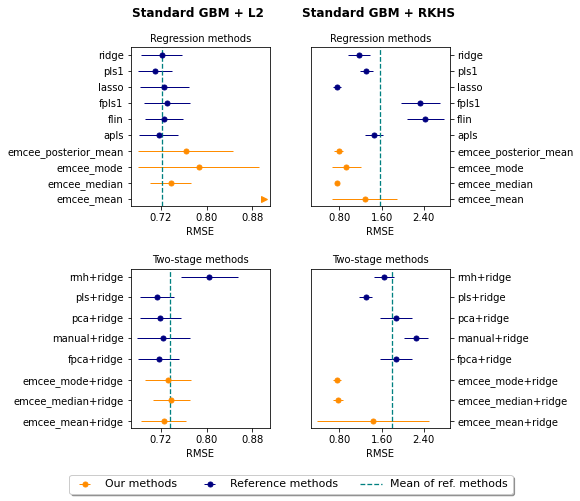
\includegraphics[width=.6\textwidth]{reg_emcee_nongp}
    \caption{Mean and standard error of RMSE of predictors (lower is better) for 10 runs with GBM regressors. In the first column the response obeys a linear \(L^2\)-model, while in the second columns it follows a RKHS linear model. The first row are direct methods and the second are dimensionality reduction methods.}\label{fig:reg_emcee_nongp}
\end{figure}

\subsubsection*{Functional logistic regression}

We consider a ``mixture'' situation in which we combine regressors from two different GPs with equal probability and label them according to their origin. Firstly, we consider a homoscedastic case to distinguish between a standard Brownian motion and a Brownian motion with a mean function that is zero until \(t=0.5\), and then becomes \(m(t)=0.75t\). Secondly, we consider a heteroscedastic case to distinguish between a standard Brownian motion and a Brownian motion with variance 2, that is, with kernel \(K(t,s)=2\min\{t,s\}\). Figure~\ref{fig:clf_emcee_nongp} shows that our classifiers perform better than most comparison algorithms when separating two homoscedastic Gaussian processes, but they struggle in the heteroscedastic case. Incidentally, this heteroscedastic case of two zero-mean Brownian motions has a special interest, since it can be shown that the Bayes error is zero in the limit of dense monitoring (i.e.\ with an arbitrarily fine measurement grid), a manifestation of the ``near-perfect'' classification phenomenon analyzed for example in \citet{torrecilla2020optimal}. Our results are in line with the empirical studies of this article, where the authors conclude that even though the asymptotic theoretical error is zero, most classification methods are suboptimal in practice (possibly due to the high collinearity of the data), with the notable exception of PCA+QDA.

\begin{figure}[ht!]
    \centering
    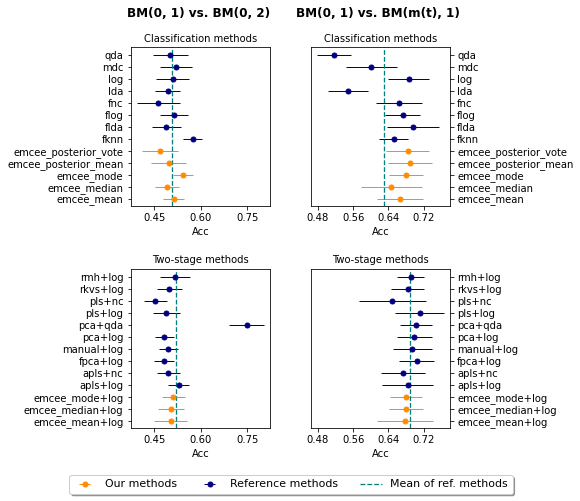
\includegraphics[width=.6\textwidth]{clf_emcee_nongp}
    \caption{Mean and standard error of accuracy of classifiers (higher is better) for 10 runs with a mix of regressors coming from two different GPs and labeled according to their origin. In the first column we try to separate two Brownian motions with the same mean but different variance, while in the second column we discriminate between two Brownian motions with different mean functions but the same variance. The first row are direct methods and the second are dimensionality reduction methods.}\label{fig:clf_emcee_nongp}
\end{figure}

\subsection{Model misspecification}

One requirement that our model should satisfy is that it ought to be able to recover the true parameter function when the underlying data generation model is a finite-dimensional RKHS model. This is generally the case when the value of \(p\) in our model and the true value \(p_0\) coincide, but what happens when we change the value of \(p\) in the model? Take for example a RKHS data set with two components generated according to the formula \(Y=5 -5X(0.1) + 10X(0.8) + \epsilon\), with \(\epsilon\sim \mathcal N(0, 0.5)\). Figure~\ref{fig:beta_trace_3} shows the resulting posterior distribution of the parameters \(b=(\beta_1, \beta_2, \beta_3)\) and \(\tau=(t_1, t_2, t_3)\) for a model with 3 components. As we can see, one of the coefficients has gone to zero to account for the overspecification of the model, while the other two have stabilized very close to the true parameters. The same goes for the time instants, except that in this case there is no default value to represent that a component is unused, so the time corresponding to the null coefficient oscillates back and forth. Note that the estimated function (based for example in the mode of the posterior distributions) will not be perfect, essentially because of the noise in the response. But it should be close to the true parameter function \(\alpha(t)=-5K(t, 0.1) + 10K(t, 0.8)\), providing a good predictive performance in most cases.

\begin{figure}[ht!]
    \centering
    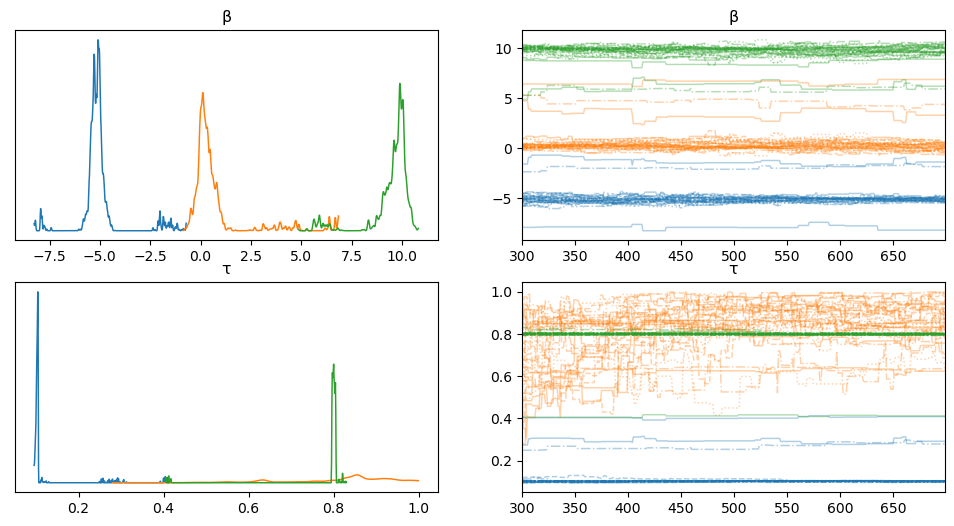
\includegraphics[width=.8\textwidth]{beta_trace_3}
    \caption{Left: estimated posterior distribution for the parameters \(b\) and \(\tau\) using our RKHS linear regression model with \(p=3\), in a linear dataset with \(p_0=2\) components. Right: the corresponding trace evolution for 400 iterations in the MCMC sampler.}\label{fig:beta_trace_3}
\end{figure}

In contrast, if we consider now a model with \(p=4\) with the same data, we might obtain posterior distributions like the ones in Figure~\ref{fig:beta_trace_4}. In this situation two coefficients should go to zero, but that is no longer the case. For example, while the green component has a high density around 0, it also has a considerable mass around 10, effectively ``competing'' with the red component. This is a manifestation of the label switching issue, caused in this case by an excessive number of degrees of freedom in the model. There is still another possible situation, one in which no label switching occurs but the estimated function has four non-negligible components. This can happen because the different components exploit the additional freedom and ``work together'', so to speak. In this way we might obtain an estimate that does not resemble the true coefficient function, but that has a very low prediction error. However, this could also work to our detriment and cause the estimated function to be worse prediction-wise than simpler alternatives. This phenomenon is expected to strengthen as the difference between the true and assumed value of \(p\) grows larger.

\begin{figure}[ht!]
    \centering
    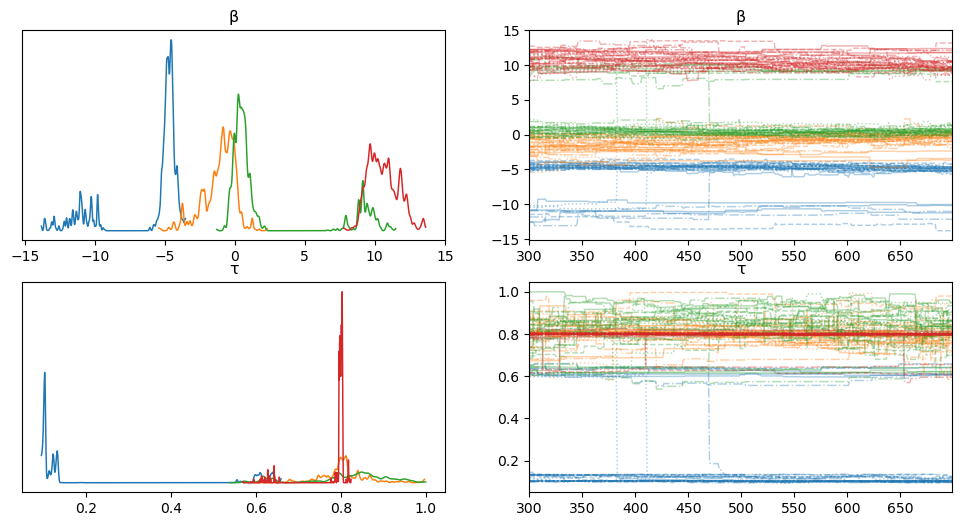
\includegraphics[width=.8\textwidth]{beta_trace_4}
    \caption{Left: estimated posterior distribution for the parameters \(b\) and \(\tau\) using our RKHS linear regression model with \(p=4\), in a linear dataset with \(p_0=2\) components. Right: the corresponding trace evolution for 400 iterations in the MCMC sampler.}\label{fig:beta_trace_4}
\end{figure}

\subsection{Dependence on the number of components}

Another thing we wanted to look at was the dependence of the final prediction result on the chosen value of \(p\), especially when there is no concept of ``components'' in the underlying model. We can take for example the homoscedastic mixture data set described in Appendix~\ref{app:non-gp} for the logistic regression problem, and fix the parameter \(\eta=0.01\). The corresponding mean accuracies (in 10 repetitions) for RKHS models with \(p=1,2,\dots 10\) components are shown in Figure~\ref{fig:dependence_acc_p}, along with their standard errors (which are arguably not very informative). It would appear that the methods that use the whole posterior distribution (\textit{emcee\_posterior\_mean} and \textit{emcee\_posterior\_vote}) are more stable and somewhat independent of the value of \(p>1\) in terms of accuracy. On the other hand, the rest of the algorithms show a slight downward trend as \(p\) increases (although not so much in the variable selection methods), and in general their best results are obtained at \(p=2\). We expect that this effect or some small variation of it will remain valid in other situations, and it would be in line with our view that the RKHS models work best with fewer components. However, a profound study of this would be the subject of a different experiment altogether.

\begin{figure}[ht!]
    \centering
    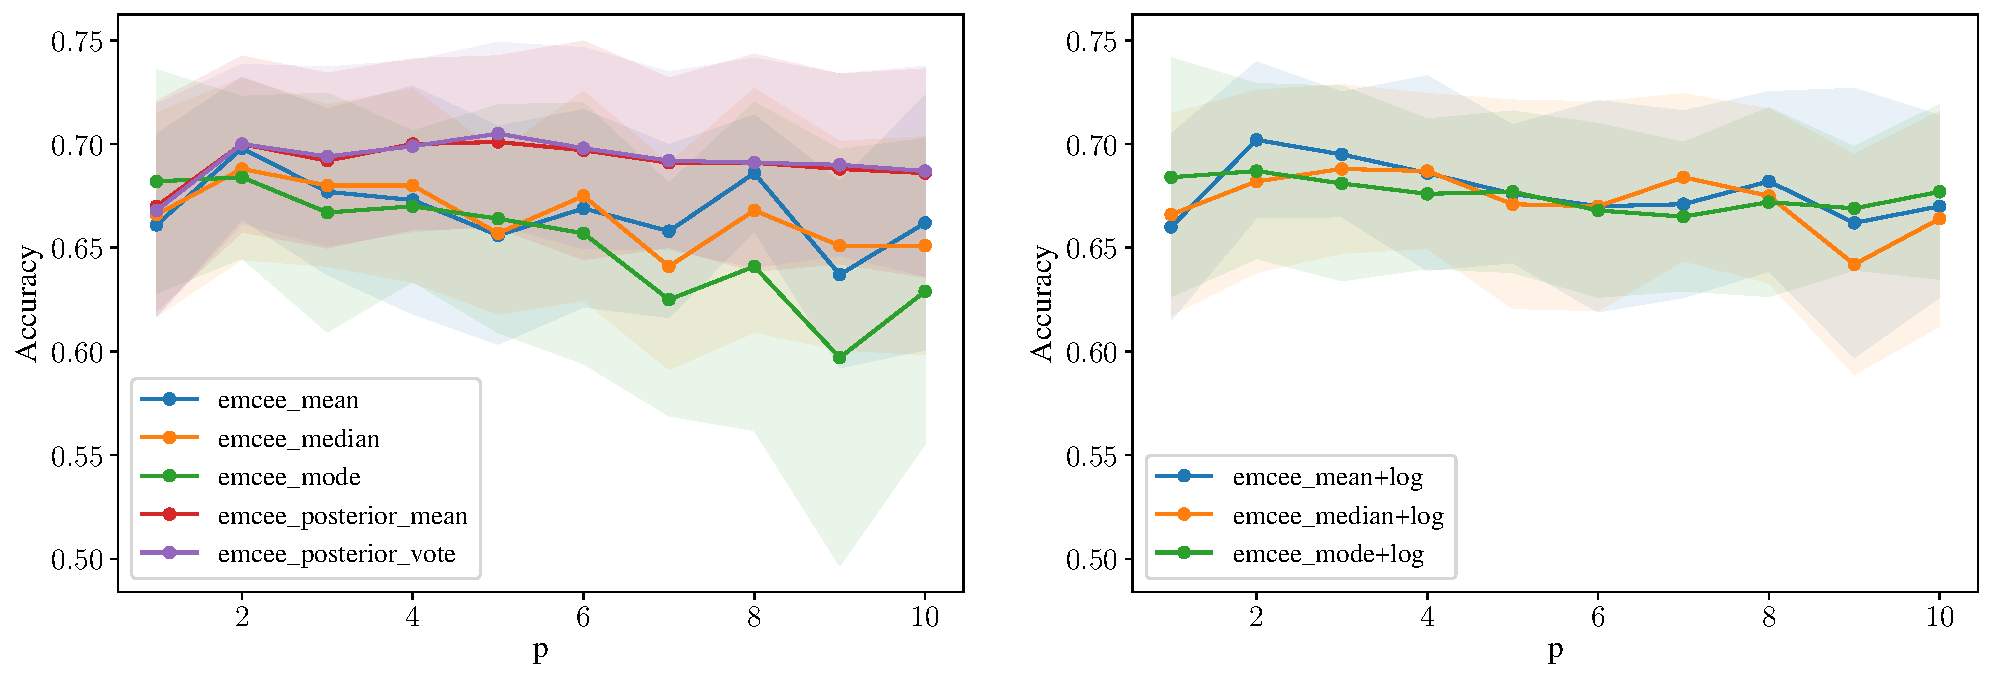
\includegraphics[width=0.85\textwidth]{mixture_dependence_acc_p}
    \caption{Mean accuracy in 10 independent repetitions for our logistic RKHS methods as a function of \(p\), using \(\eta=0.01\) and the homoscedastic mixture data set. The corresponding standard errors are shown in faded colors.}\label{fig:dependence_acc_p}
\end{figure}


\subsection{Tables of experimental results}\label{app:tables}

We present below the tables corresponding to the empirical comparison studies in Appendix~\ref{app:non-gp} and in Section~\ref{sec:results}, which show the numerical values that were depicted there graphically. In each case the best and second-best results are shown in \firstcolor{bold} and \secondcolor{italics}, respectively.

\subsubsection*{Functional linear regression}

\begin{table}[htbp!]
    \footnotesize
    \centering
    \rowcolors{2}{}{teal!8}
    \begin{tabular}{lcccc}
        \toprule
        \textbf{Prediction method} & \textbf{BM}                 & \textbf{fBM}                & \textbf{O-U}                & \textbf{Gaussian}           \\
        \midrule
        emcee\_mean                & 0.913 (0.310)               & 0.759 (0.068)               & 0.806 (0.098)               & 1.408 (1.359)               \\
        emcee\_median              & \secondcolor{0.729 (0.048)} & \secondcolor{0.729 (0.045)} & \secondcolor{0.740 (0.052)} & 0.743 (0.041)               \\
        emcee\_mode                & 0.735 (0.039)               & 0.748 (0.068)               & 0.769 (0.102)               & 0.803 (0.147)               \\
        emcee\_posterior\_mean     & 0.743 (0.047)               & \firstcolor{0.726 (0.036)}  & 0.863 (0.416)               & 0.766 (0.061)               \\
        apls                       & 1.003 (0.045)               & 0.792 (0.030)               & 1.167 (0.068)               & \secondcolor{0.728 (0.035)} \\
        flin                       & 1.219 (0.056)               & 0.800 (0.022)               & 1.630 (0.051)               & 0.738 (0.030)               \\
        fpls1                      & 1.235 (0.069)               & 0.800 (0.024)               & 1.631 (0.053)               & 0.738 (0.035)               \\
        lasso                      & \firstcolor{0.727 (0.034)}  & 0.738 (0.027)               & \firstcolor{0.731 (0.039)}  & \firstcolor{0.726 (0.032)}  \\
        pls1                       & 1.032 (0.116)               & 0.782 (0.034)               & 0.974 (0.063)               & 0.729 (0.041)               \\
        ridge                      & 0.920 (0.043)               & 0.778 (0.021)               & 0.965 (0.059)               & \secondcolor{0.728 (0.035)} \\

        \bottomrule
        \toprule

        emcee\_mean+ridge          & 0.816 (0.154)               & 0.749 (0.044)               & \secondcolor{0.734 (0.039)} & 0.799 (0.175)               \\
        emcee\_median+ridge        & \secondcolor{0.759 (0.063)} & \secondcolor{0.741 (0.041)} & 0.751 (0.065)               & 0.755 (0.058)               \\
        emcee\_mode+ridge          & \firstcolor{0.746 (0.058)}  & \firstcolor{0.735 (0.036)}  & \firstcolor{0.726 (0.038)}  & 0.735 (0.036)               \\
        fpca+ridge                 & 1.149 (0.041)               & 0.784 (0.020)               & 1.420 (0.063)               & \secondcolor{0.728 (0.033)} \\
        manual+ridge               & 1.221 (0.050)               & 0.784 (0.021)               & 1.548 (0.072)               & \firstcolor{0.727 (0.032)}  \\
        pca+ridge                  & 1.153 (0.041)               & 0.784 (0.022)               & 1.422 (0.050)               & 0.730 (0.033)               \\
        pls+ridge                  & 0.955 (0.053)               & 0.783 (0.031)               & 0.962 (0.059)               & 0.729 (0.035)               \\
        rmh+ridge                  & 1.423 (0.117)               & 0.847 (0.043)               & 1.375 (0.266)               & 1.226 (0.117)               \\

        \bottomrule
    \end{tabular}
    \caption{Mean RMSE of predictors (lower is better) for 10 runs with GP regressors, one in each column, that obey an underlying linear RKHS model. The corresponding standard errors are shown between brackets.}
\end{table}
\newpage
\FloatBarrier{}

\begin{table}[htbp!]
    \vspace{.5em}
    \footnotesize
    \centering
    \rowcolors{2}{}{teal!8}
    \begin{tabular}{lcccc}
        \toprule
        \textbf{Prediction method} & \textbf{BM}                 & \textbf{fBM}                & \textbf{O-U}                & \textbf{Gaussian}           \\
        \midrule
        emcee\_mean                & 0.769 (0.037)               & 0.744 (0.061)               & 0.756 (0.054)               & 0.794 (0.129)               \\
        emcee\_median              & 0.730 (0.049)               & 0.751 (0.071)               & 0.718 (0.031)               & \firstcolor{0.722 (0.030)}  \\
        emcee\_mode                & 0.732 (0.032)               & 0.739 (0.075)               & 0.730 (0.038)               & 0.730 (0.029)               \\
        emcee\_posterior\_mean     & 0.723 (0.040)               & 0.720 (0.032)               & 0.755 (0.079)               & \secondcolor{0.726 (0.026)} \\
        apls                       & \secondcolor{0.715 (0.030)} & \firstcolor{0.710 (0.030)}  & \firstcolor{0.710 (0.029)}  & \secondcolor{0.726 (0.031)} \\
        flin                       & 0.733 (0.035)               & 0.727 (0.033)               & 0.733 (0.035)               & 0.735 (0.032)               \\
        fpls1                      & 0.718 (0.039)               & 0.726 (0.035)               & 0.731 (0.034)               & \secondcolor{0.726 (0.033)} \\
        lasso                      & \firstcolor{0.712 (0.027)}  & \secondcolor{0.712 (0.028)} & 0.717 (0.029)               & \firstcolor{0.722 (0.029)}  \\
        pls1                       & 0.717 (0.041)               & 0.720 (0.036)               & 0.722 (0.029)               & 0.729 (0.031)               \\
        ridge                      & 0.716 (0.029)               & 0.717 (0.032)               & \secondcolor{0.716 (0.032)} & 0.727 (0.033)               \\
        \bottomrule
        \toprule
        emcee\_mean+ridge          & \firstcolor{0.717 (0.029)}  & \secondcolor{0.718 (0.030)} & 0.719 (0.027)               & 0.743 (0.052)               \\
        emcee\_median+ridge        & 0.722 (0.038)               & 0.723 (0.038)               & \secondcolor{0.717 (0.035)} & 0.730 (0.025)               \\
        emcee\_mode+ridge          & 0.726 (0.036)               & 0.735 (0.048)               & 0.736 (0.030)               & 0.743 (0.050)               \\
        fpca+ridge                 & \firstcolor{0.717 (0.032)}  & \secondcolor{0.718 (0.030)} & 0.718 (0.033)               & \firstcolor{0.727 (0.031)}  \\
        manual+ridge               & \firstcolor{0.717 (0.030)}  & 0.719 (0.030)               & \firstcolor{0.716 (0.032)}  & \secondcolor{0.728 (0.031)} \\
        pca+ridge                  & \firstcolor{0.717 (0.032)}  & 0.720 (0.031)               & \firstcolor{0.716 (0.032)}  & \firstcolor{0.727 (0.031)}  \\
        pls+ridge                  & \secondcolor{0.719 (0.033)} & 0.728 (0.046)               & 0.720 (0.033)               & 0.730 (0.031)               \\
        rmh+ridge                  & 0.753 (0.029)               & \firstcolor{0.713 (0.030)}  & 0.791 (0.037)               & 0.812 (0.027)               \\
        \bottomrule
    \end{tabular}
    \caption{Mean RMSE of predictors (lower is better) for 10 runs with GP regressors, one in each column, that obey an underlying linear \(L^2\)-model. The corresponding standard errors are shown between brackets.}
\end{table}

\vspace{2em}

\begin{table}[htbp!]
    \footnotesize
    \centering
    \rowcolors{2}{}{teal!8}
    \begin{tabular}{lcc}
        \toprule
        \textbf{Prediction method} & \textbf{GBM + \(\bf{L^2}\)} & \textbf{GBM + RKHS}         \\
        \midrule
        emcee\_mean                & 0.948 (0.354)               & 1.278 (0.622)               \\
        emcee\_median              & 0.737 (0.036)               & \firstcolor{0.747 (0.031)}  \\
        emcee\_mode                & 0.786 (0.106)               & 0.928 (0.275)               \\
        emcee\_posterior\_mean     & 0.763 (0.083)               & 0.786 (0.084)               \\
        apls                       & \secondcolor{0.716 (0.034)} & 1.456 (0.170)               \\
        flin                       & 0.726 (0.033)               & 2.427 (0.352)               \\
        fpls1                      & 0.731 (0.040)               & 2.336 (0.365)               \\
        lasso                      & 0.726 (0.042)               & \secondcolor{0.759 (0.073)} \\
        pls1                       & \firstcolor{0.710 (0.029)}  & 1.309 (0.122)               \\
        ridge                      & 0.721 (0.035)               & 1.175 (0.205)               \\

        \bottomrule
        \toprule
        emcee\_mean+ridge          & 0.725 (0.040)               & 1.432 (1.059)               \\
        emcee\_median+ridge        & 0.738 (0.033)               & \secondcolor{0.780 (0.093)} \\
        emcee\_mode+ridge          & 0.733 (0.040)               & \firstcolor{0.760 (0.073)}  \\
        fpca+ridge                 & \secondcolor{0.716 (0.036)} & 1.873 (0.302)               \\
        manual+ridge               & 0.724 (0.046)               & 2.253 (0.226)               \\
        pca+ridge                  & 0.719 (0.036)               & 1.879 (0.304)               \\
        pls+ridge                  & \firstcolor{0.713 (0.030)}  & 1.299 (0.125)               \\
        rmh+ridge                  & 0.805 (0.051)               & 1.640 (0.189)               \\

        \bottomrule
    \end{tabular}
    \caption{Mean RMSE of predictors (lower is better) for 10 runs with GBM regressors. In the first column the response obeys a linear \(L^2\)-model, while in the second column it follows a RKHS linear model. The corresponding standard errors are shown between brackets.}
\end{table}
\newpage
\FloatBarrier{}

\begin{table}[htbp!]
    \vspace{.5em}
    \footnotesize
    \centering
    \rowcolors{2}{}{teal!8}
    \begin{tabular}{lccc}
        \toprule
        \textbf{Prediction method} & \textbf{Moisture}           & \textbf{Sugar}              & \textbf{Tecator}            \\
        \midrule
        emcee\_mean                & 1.268 (1.096)               & 9.207 (9.248)               & 9.811 (7.446)               \\
        emcee\_median              & 0.296 (0.051)               & 3.130 (2.584)               & 3.714 (0.922)               \\
        emcee\_mode                & 0.301 (0.049)               & 2.628 (0.700)               & 3.531 (1.494)               \\
        emcee\_posterior\_mean     & 0.255 (0.039)               & 2.813 (0.897)               & 2.918 (0.222)               \\
        flin                       & 0.257 (0.026)               & 1.978 (0.210)               & \secondcolor{2.604 (0.344)} \\
        fpls1                      & 0.236 (0.038)               & 1.993 (0.223)               & \secondcolor{2.604 (0.294)} \\
        lasso                      & 0.242 (0.028)               & \secondcolor{1.975 (0.199)} & 2.892 (0.270)               \\
        pls1                       & \secondcolor{0.228 (0.023)} & 2.045 (0.190)               & 2.704 (0.467)               \\
        ridge                      & \firstcolor{0.221 (0.026)}  & \firstcolor{1.952 (0.235)}  & 3.387 (0.218)               \\
        apls                       & 0.234 (0.031)               & 2.050 (0.238)               & \firstcolor{2.349 (0.470)}  \\
        \bottomrule
        \toprule
        emcee\_mean+ridge          & 0.262 (0.043)               & 2.020 (0.198)               & 6.673 (1.037)               \\
        emcee\_median+ridge        & 0.260 (0.034)               & 1.995 (0.219)               & 5.393 (1.210)               \\
        emcee\_mode+ridge          & 0.302 (0.092)               & 2.037 (0.200)               & 5.442 (0.563)               \\
        fpca+ridge                 & 0.289 (0.035)               & \secondcolor{1.976 (0.227)} & 9.521 (0.603)               \\
        manual+ridge               & \secondcolor{0.228 (0.026)} & 1.987 (0.227)               & 4.126 (0.305)               \\
        pca+ridge                  & \firstcolor{0.226 (0.027)}  & \firstcolor{1.963 (0.234)}  & \secondcolor{3.388 (0.218)} \\
        pls+ridge                  & \firstcolor{0.226 (0.025)}  & 2.012 (0.218)               & \firstcolor{2.415 (0.501)}  \\
        rmh+ridge                  & 0.327 (0.086)               & 2.031 (0.216)               & 5.580 (0.513)               \\
        \bottomrule
    \end{tabular}
    \caption{Mean RMSE of predictors (lower is better) for 10 runs with real data sets, one in each column. The corresponding standard errors are shown between brackets.}
\end{table}
\newpage
\FloatBarrier{}

\subsubsection*{Functional logistic regression}

\begin{table}[htbp!]
    \footnotesize
    \centering
    \rowcolors{2}{}{teal!8}
    \begin{tabular}{lcccc}
        \toprule
        \textbf{Classification method} & \textbf{BM}                 & \textbf{fBM}                & \textbf{O-U}                & \textbf{Gaussian}           \\
        \midrule
        emcee\_mean                    & 0.743 (0.052)               & 0.739 (0.040)               & 0.734 (0.029)               & 0.751 (0.039)               \\
        emcee\_median                  & 0.771 (0.048)               & 0.716 (0.048)               & 0.714 (0.049)               & 0.746 (0.055)               \\
        emcee\_mode                    & \secondcolor{0.777 (0.037)} & 0.752 (0.043)               & 0.724 (0.029)               & 0.760 (0.048)               \\
        emcee\_posterior\_mean         & 0.764 (0.044)               & 0.756 (0.046)               & 0.734 (0.029)               & 0.753 (0.040)               \\
        emcee\_posterior\_vote         & 0.765 (0.043)               & 0.753 (0.040)               & \secondcolor{0.747 (0.027)} & 0.753 (0.043)               \\
        fknn                           & 0.765 (0.027)               & \secondcolor{0.768 (0.033)} & 0.743 (0.032)               & 0.738 (0.022)               \\
        flda                           & 0.767 (0.055)               & 0.755 (0.048)               & 0.735 (0.036)               & \secondcolor{0.761 (0.050)} \\
        flog                           & 0.771 (0.033)               & 0.761 (0.042)               & 0.745 (0.025)               & \firstcolor{0.777 (0.040)}  \\
        fnc                            & 0.743 (0.029)               & \firstcolor{0.775 (0.042)}  & 0.661 (0.063)               & 0.755 (0.035)               \\
        lda                            & 0.514 (0.054)               & 0.601 (0.030)               & 0.578 (0.032)               & 0.702 (0.059)               \\
        log                            & \firstcolor{0.778 (0.031)}  & 0.750 (0.042)               & \firstcolor{0.761 (0.039)}  & \secondcolor{0.761 (0.031)} \\
        mdc                            & 0.724 (0.033)               & 0.762 (0.037)               & 0.648 (0.052)               & 0.732 (0.023)               \\
        qda                            & 0.499 (0.038)               & 0.488 (0.041)               & 0.472 (0.055)               & 0.483 (0.027)               \\

        \bottomrule
        \toprule

        emcee\_mean+logistic           & 0.781 (0.036)               & 0.746 (0.038)               & 0.725 (0.051)               & 0.750 (0.034)               \\
        emcee\_median+logistic         & 0.766 (0.041)               & 0.749 (0.045)               & 0.717 (0.024)               & 0.732 (0.066)               \\
        emcee\_mode+logistic           & 0.776 (0.042)               & 0.746 (0.047)               & 0.726 (0.025)               & 0.761 (0.036)               \\
        apls+log                       & \secondcolor{0.783 (0.025)} & 0.756 (0.036)               & 0.739 (0.020)               & 0.761 (0.028)               \\
        apls+nc                        & 0.771 (0.048)               & 0.745 (0.045)               & 0.740 (0.022)               & 0.751 (0.034)               \\
        fpca+log                       & 0.773 (0.028)               & 0.755 (0.038)               & \firstcolor{0.758 (0.032)}  & 0.765 (0.039)               \\
        manual+log                     & 0.753 (0.033)               & 0.758 (0.040)               & 0.742 (0.031)               & 0.754 (0.032)               \\
        pca+log                        & 0.780 (0.032)               & 0.758 (0.036)               & \secondcolor{0.756 (0.032)} & 0.756 (0.033)               \\
        pca+qda                        & 0.751 (0.037)               & 0.750 (0.049)               & 0.736 (0.019)               & 0.741 (0.030)               \\
        pls+log                        & \firstcolor{0.786 (0.040)}  & \firstcolor{0.768 (0.037)}  & 0.740 (0.035)               & 0.766 (0.033)               \\
        pls+nc                         & 0.744 (0.032)               & \secondcolor{0.766 (0.039)} & 0.745 (0.055)               & 0.767 (0.035)               \\
        rkvs+log                       & 0.770 (0.037)               & 0.757 (0.040)               & 0.738 (0.026)               & \secondcolor{0.772 (0.039)} \\
        rmh+log                        & 0.768 (0.047)               & 0.760 (0.043)               & 0.745 (0.019)               & \firstcolor{0.781 (0.036)}  \\
        \bottomrule
    \end{tabular}
    \caption{Mean accuracy of classifiers (higher is better) for 10 runs with GP regressors, one in each column, that obey an underlying logistic RKHS model. The corresponding standard errors are shown between brackets.}
\end{table}
\newpage
\FloatBarrier{}

\begin{table}[htbp!]
    \vspace{.5em}
    \footnotesize
    \centering
    \rowcolors{2}{}{teal!8}
    \begin{tabular}{lcccc}
        \toprule
        \textbf{Classification method} & \textbf{BM}                 & \textbf{fBM}                & \textbf{O-U}                & \textbf{Gaussian}           \\
        \midrule

        emcee\_mean                    & 0.571 (0.053)               & \secondcolor{0.557 (0.037)} & \firstcolor{0.594 (0.021)}  & 0.565 (0.082)               \\
        emcee\_median                  & 0.557 (0.033)               & 0.539 (0.045)               & 0.559 (0.059)               & 0.556 (0.049)               \\
        emcee\_mode                    & 0.553 (0.063)               & 0.513 (0.067)               & 0.575 (0.038)               & 0.550 (0.042)               \\
        emcee\_posterior\_mean         & 0.575 (0.049)               & \firstcolor{0.560 (0.036)}  & \secondcolor{0.593 (0.022)} & \firstcolor{0.578 (0.039)}  \\
        emcee\_posterior\_vote         & 0.576 (0.034)               & 0.554 (0.039)               & 0.579 (0.023)               & \secondcolor{0.576 (0.041)} \\
        fknn                           & 0.557 (0.022)               & 0.505 (0.047)               & 0.576 (0.042)               & 0.557 (0.026)               \\
        flda                           & 0.554 (0.032)               & 0.516 (0.053)               & 0.543 (0.057)               & 0.526 (0.049)               \\
        flog                           & 0.587 (0.034)               & 0.542 (0.036)               & 0.576 (0.038)               & \firstcolor{0.578 (0.043)}  \\
        fnc                            & \secondcolor{0.601 (0.036)} & 0.545 (0.045)               & 0.587 (0.037)               & 0.546 (0.056)               \\
        lda                            & 0.507 (0.041)               & 0.482 (0.056)               & 0.524 (0.042)               & 0.525 (0.052)               \\
        log                            & 0.576 (0.034)               & 0.546 (0.033)               & 0.560 (0.053)               & 0.554 (0.037)               \\
        mdc                            & \firstcolor{0.605 (0.039)}  & 0.544 (0.055)               & 0.584 (0.039)               & 0.533 (0.042)               \\
        qda                            & 0.476 (0.050)               & 0.518 (0.048)               & 0.470 (0.071)               & 0.485 (0.039)               \\

        \bottomrule
        \toprule
        emcee\_mean+logistic           & \firstcolor{0.583 (0.038)}  & \firstcolor{0.575 (0.043)}  & 0.569 (0.021)               & 0.559 (0.030)               \\
        emcee\_median+logistic         & 0.565 (0.044)               & 0.552 (0.037)               & \secondcolor{0.589 (0.029)} & \firstcolor{0.585 (0.041)}  \\
        emcee\_mode+logistic           & 0.568 (0.047)               & 0.544 (0.036)               & 0.581 (0.041)               & 0.557 (0.033)               \\
        apls+log                       & 0.556 (0.066)               & 0.535 (0.040)               & 0.548 (0.070)               & 0.560 (0.055)               \\
        apls+nc                        & 0.549 (0.056)               & 0.523 (0.040)               & 0.545 (0.054)               & 0.545 (0.047)               \\
        fpca+log                       & 0.559 (0.037)               & 0.548 (0.033)               & 0.579 (0.034)               & 0.564 (0.032)               \\
        manual+log                     & 0.573 (0.037)               & 0.542 (0.029)               & 0.575 (0.043)               & 0.568 (0.035)               \\
        pca+log                        & 0.570 (0.036)               & 0.541 (0.033)               & 0.579 (0.028)               & 0.567 (0.033)               \\
        pca+qda                        & 0.567 (0.030)               & 0.532 (0.045)               & 0.577 (0.037)               & 0.574 (0.059)               \\
        pls+log                        & 0.564 (0.042)               & 0.556 (0.028)               & 0.559 (0.041)               & 0.564 (0.036)               \\
        pls+nc                         & \secondcolor{0.581 (0.038)} & 0.535 (0.048)               & \secondcolor{0.589 (0.043)} & 0.558 (0.057)               \\
        rkvs+log                       & 0.572 (0.058)               & 0.550 (0.023)               & \firstcolor{0.592 (0.018)}  & 0.567 (0.024)               \\
        rmh+log                        & 0.570 (0.036)               & \secondcolor{0.557 (0.033)} & 0.584 (0.024)               & \secondcolor{0.581 (0.025)} \\
        \bottomrule
    \end{tabular}
    \caption{Mean accuracy of classifiers (higher is better) for 10 runs with GP regressors, one in each column, that obey an underlying logistic \(L^2\)-model. The corresponding standard errors are shown between brackets.}
\end{table}
\newpage
\FloatBarrier{}

\begin{table}[htbp!]
    \vspace{.5em}
    \footnotesize
    \centering
    \rowcolors{2}{}{teal!8}
    \begin{tabular}{lcccc}
        \toprule
        \textbf{Classification method} & \textbf{Heteroscedastic}    & \textbf{Homoscedastic}      \\
        \midrule

        emcee\_mean                    & 0.513 (0.035)               & 0.667 (0.053)               \\
        emcee\_median                  & 0.492 (0.039)               & 0.647 (0.070)               \\
        emcee\_mode                    & \secondcolor{0.543 (0.033)} & 0.680 (0.038)               \\
        emcee\_posterior\_mean         & 0.497 (0.056)               & \secondcolor{0.690 (0.050)} \\
        emcee\_posterior\_vote         & 0.469 (0.058)               & 0.684 (0.048)               \\
        fknn                           & \firstcolor{0.574 (0.031)}  & 0.652 (0.034)               \\
        flda                           & 0.489 (0.047)               & \firstcolor{0.696 (0.059)}  \\
        flog                           & 0.515 (0.045)               & 0.673 (0.040)               \\
        fnc                            & 0.463 (0.069)               & 0.664 (0.053)               \\
        lda                            & 0.493 (0.040)               & 0.548 (0.046)               \\
        log                            & 0.509 (0.055)               & 0.686 (0.046)               \\
        mdc                            & 0.521 (0.052)               & 0.601 (0.058)               \\
        qda                            & 0.502 (0.056)               & 0.517 (0.039)               \\

        \bottomrule
        \toprule

        emcee\_mean+logistic           & 0.503 (0.054)               & 0.678 (0.063)               \\
        emcee\_median+logistic         & 0.504 (0.041)               & 0.680 (0.038)               \\
        emcee\_mode+logistic           & 0.512 (0.036)               & 0.681 (0.036)               \\
        apls+log                       & \secondcolor{0.529 (0.034)} & 0.684 (0.058)               \\
        apls+nc                        & 0.496 (0.039)               & 0.674 (0.050)               \\
        fpca+log                       & 0.481 (0.032)               & \secondcolor{0.704 (0.041)} \\
        manual+log                     & 0.496 (0.029)               & 0.694 (0.044)               \\
        pca+log                        & 0.483 (0.030)               & 0.699 (0.040)               \\
        pca+qda                        & \firstcolor{0.748 (0.055)}  & 0.703 (0.037)               \\
        pls+log                        & 0.489 (0.043)               & \firstcolor{0.711 (0.055)}  \\
        pls+nc                         & 0.454 (0.037)               & 0.649 (0.076)               \\
        rkvs+log                       & 0.499 (0.041)               & 0.684 (0.037)               \\
        rmh+log                        & 0.516 (0.049)               & 0.691 (0.030)               \\

        \bottomrule
    \end{tabular}
    \caption{Mean accuracy of classifiers (higher is better) for 10 runs with a mix of regressors coming from two different GPs and labeled according to their origin. In the first column we try to separate two heteroscedastic Brownian motions, while in the second column we discriminate between two homoscedastic Brownian motions. The corresponding standard errors are shown between brackets.}
\end{table}
\newpage
\FloatBarrier{}

\begin{table}[htbp!]
    \vspace{.5em}
    \footnotesize
    \centering
    \rowcolors{2}{}{teal!8}
    \begin{tabular}{lcccc}
        \toprule
        \textbf{Classification method} & \textbf{Growth}             & \textbf{Medflies}           & \textbf{Phoneme}            \\
        \midrule

        emcee\_mean                    & 0.858 (0.147)               & 0.533 (0.041)               & 0.763 (0.041)               \\
        emcee\_median                  & 0.894 (0.112)               & 0.573 (0.032)               & 0.776 (0.044)               \\
        emcee\_mode                    & 0.932 (0.034)               & 0.582 (0.034)               & 0.770 (0.056)               \\
        emcee\_posterior\_mean         & 0.926 (0.032)               & \secondcolor{0.596 (0.044)} & 0.797 (0.035)               \\
        emcee\_posterior\_vote         & 0.919 (0.046)               & 0.575 (0.052)               & \secondcolor{0.801 (0.031)} \\
        fknn                           & 0.942 (0.040)               & 0.534 (0.031)               & 0.760 (0.046)               \\
        flda                           & \secondcolor{0.945 (0.032)} & 0.561 (0.020)               & 0.781 (0.037)               \\
        flog                           & 0.935 (0.050)               & \firstcolor{0.601 (0.029)}  & 0.766 (0.041)               \\
        fnc                            & 0.735 (0.112)               & 0.546 (0.038)               & 0.703 (0.036)               \\
        lda                            & 0.894 (0.052)               & 0.572 (0.019)               & 0.618 (0.040)               \\
        log                            & \firstcolor{0.965 (0.030)}  & 0.575 (0.028)               & \firstcolor{0.822 (0.026)}  \\
        mdc                            & 0.700 (0.087)               & 0.524 (0.026)               & 0.663 (0.031)               \\
        qda                            & 0.581 (0.000)               & 0.569 (0.023)               & 0.457 (0.043)               \\

        \bottomrule
        \toprule

        emcee\_mean+logistic           & 0.906 (0.118)               & 0.528 (0.029)               & 0.779 (0.033)               \\
        emcee\_median+logistic         & 0.932 (0.049)               & 0.580 (0.031)               & 0.796 (0.036)               \\
        emcee\_mode+logistic           & 0.935 (0.043)               & 0.585 (0.032)               & 0.791 (0.038)               \\
        apls+log                       & 0.952 (0.026)               & 0.572 (0.016)               & \firstcolor{0.816 (0.028)}  \\
        apls+nc                        & 0.952 (0.041)               & 0.554 (0.020)               & \secondcolor{0.807 (0.032)} \\
        fpca+log                       & \firstcolor{0.965 (0.030)}  & 0.551 (0.032)               & 0.797 (0.021)               \\
        manual+log                     & \secondcolor{0.961 (0.032)} & 0.584 (0.018)               & 0.778 (0.039)               \\
        pca+log                        & 0.958 (0.029)               & 0.576 (0.030)               & 0.794 (0.030)               \\
        pca+qda                        & 0.958 (0.032)               & 0.567 (0.036)               & 0.784 (0.034)               \\
        pls+log                        & 0.952 (0.036)               & 0.578 (0.018)               & 0.804 (0.031)               \\
        pls+nc                         & 0.829 (0.094)               & 0.570 (0.040)               & 0.754 (0.041)               \\
        rkvs+log                       & 0.923 (0.052)               & \secondcolor{0.596 (0.032)} & 0.796 (0.031)               \\
        rmh+log                        & 0.955 (0.030)               & \firstcolor{0.606 (0.025)}  & 0.778 (0.048)               \\

        \bottomrule
    \end{tabular}
    \caption{Mean accuracy of classifiers (higher is better) for 10 runs with real data sets, one in each column. The corresponding standard errors are shown between brackets.}
\end{table}
\newpage
\FloatBarrier{}

\section{Source code overview}\label{app:source-code}

The Python code developed for this work is available under a GPLv3 license at the GitHub repository \url{https://github.com/antcc/rk-bfr}. The code is adequately documented and is structured in several directories as follows:

\begin{itemize}
    \item In the \texttt{rkbfr} folder we find the files responsible for the implementation of our Bayesian models, separated according to the functionality they provide.
    \item The \texttt{reference\_methods} folder contains our implementation of the functional comparison algorithms that were not available through a standard Python library.
    \item The \texttt{utils} folder has some utility files for simulation, experimentation and visualization.
    \item The \texttt{experiments} folder contains plain text files with the numerical experimental results shown in Appendix~\ref{app:tables}, as well as \texttt{.csv} and \texttt{.npz} files that facilitate working with them directly in Python.
    \item At the root folder we have files for executing our experiments, which accept several user-specified parameters (such as the number of iterations or the type of data set). In particular, the script \texttt{results\_cv.py} contains the code for our comparison experiments, while the script \texttt{results\_all.py} executes our Bayesian methods without a cross-validation loop.
  \end{itemize}

When possible, the code was implemented in a generic way that would allow for easy extensions or derivations. It was also developed with efficiency in mind, so many functions and methods exploit the vectorization capabilities of the \textit{numpy} and \textit{scipy} libraries. Moreover, since we followed closely the style of the \textit{scikit-learn} and \textit{scikit-fda} libraries, our methods are compatible and could be integrated (after some minor tweaking) with both of them. The code for the experiments was executed with a random seed set to the value 2022 for reproducibility. We provide a script file \texttt{launch.sh} that illustrates a typical execution. Lastly, there are \textit{Jupyter} notebooks that demonstrate the use of our methods in a more visual way. Inside these notebooks there is a step-by-step guide on how one might execute our algorithms, accompanied by many graphical representations, and offering the possibility of changing multiple parameters to experiment with the code. In addition, there is also a notebook that can be used to generate all the tables and figures of this document pertaining to the experimental results.


%%%%%%%%%%%%%%%%%%%%%%%%%%%%%%%%%%%%%%%%%%%%%%%%%%%%%%%%%%%%%%%%%%